


%\begin{figure}[t] \centering
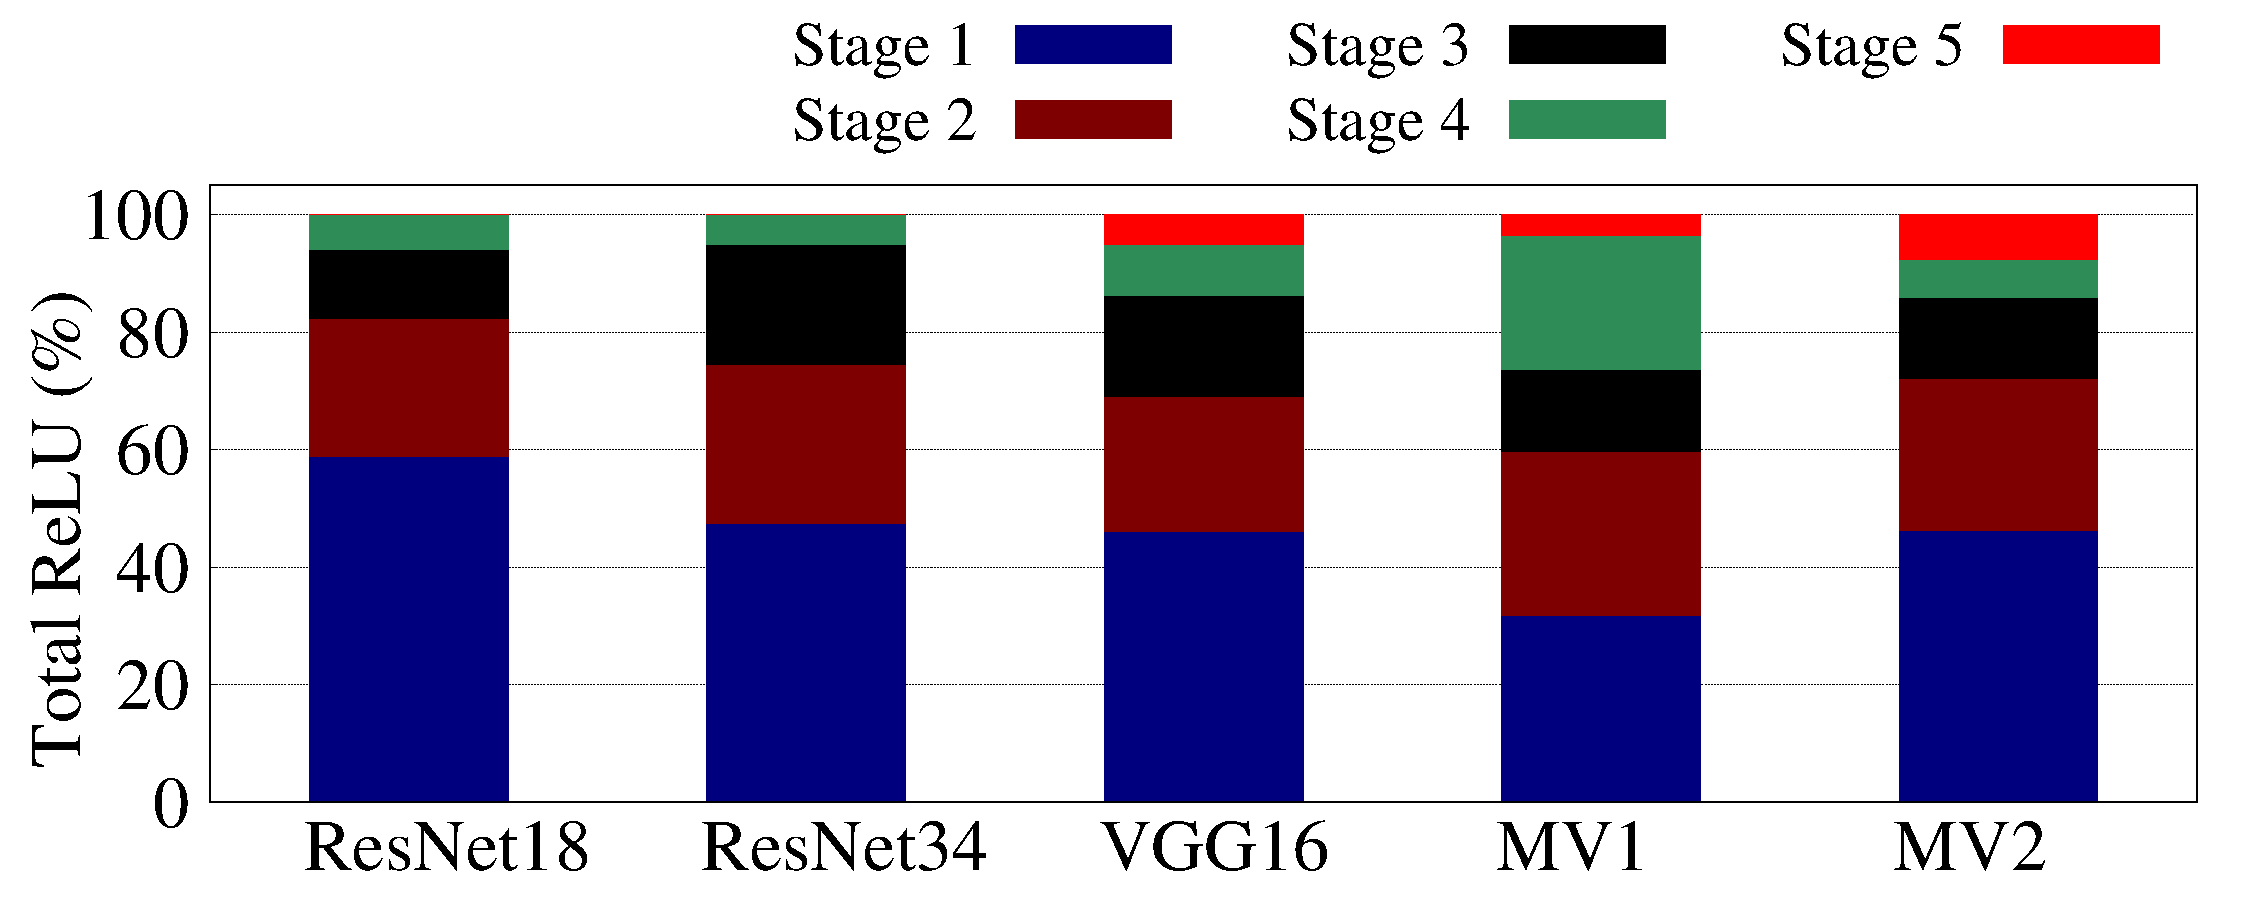
\includegraphics[scale=0.225]{Figures/StageWiseReluPercentage}
\vspace{-2em}
\caption{Stage-wise ReLU distribution in CNNs: MV1/MV2 is MobileNetV1/V2.
We note most ReLUs go to the initial stages.}
\label{fig:StageWiseReluPercentage}
\end{figure}


\section{Conclusion and Future Work} \label{sec:Conclusion}
This paper develops the concept of ReLU dropping  
as an effective method for tailoring networks for private inference.
The DeepReDuce method carefully prioritizes and
removes ReLUs based on how critical they are, and users are given a
wide range of networks that trade ReLU count and accuracy.
Evaluating DeepReDuce on CIFAR-100 shows 3.5\% improvement at iso-ReLU and 3.5$\times$ ReLU reduction at iso-accuracy. 
We also perform the experiments on TinyImageNet, which is uncommon for private inference work given the long runtimes. 
While we advance the state-of-the-art, we still fall short of the ultimate goal of real-time private inference.
We expect DeepReduce to inspire future optimizations and new ways of Thinking about network design to achieve this goal.

% Even with DeepReDuce, a CIFAR-100 network with an accuracy
% of 68.7\% takes 738mS to run, far from the
% standard throughput-latency image processing benchmarks of
% 30 frames-per-second (FPS), which translates to 33mS per inference.
% Given the long run-times of private inference, it is common practice
% for private inference papers to use CIFAR10/100. 
% However,  we ran ReLU dropping optimizations on TinyImageNet and measured the inference latency for the ReLU-optimized DeepReDuce models in Table~\ref{tab:R18OnTinyImageNet}. 
% We also ran it for MobileNetV1 on CIFAR-100 and results are shown in Table \ref{tab:ReluCriticalityMV1} in Appendix. 

% To understand the potential of ReLU dropping in other model architectures, we present a breakdown of the stage-wise distribution of ReLUs for ResNets \cite{he2016deep}, VGG16 \cite{simonyan2014very}, and MobileNets \cite{howard2017mobilenets,sandler2018mobilenetv2} in Figure~\ref{fig:StageWiseReluPercentage}.
% The layer-wise distribution of ReLUs, along with the parameters and FLOPs count, are depicted in Figure \ref{fig:LayerWiseReluInOtherDNNs} in the Appendix. We find that while all of these models differ significantly, they all have a disproportionate amount of ReLUs in the early stages.
% Recall we observe that ReLUs in early layers are the easiest to drop.  Therefore, we are optimistic about DeepReDuce's ability to generalize beyond ResNet architectures.


%\input{22Table_RevisitDesignMethods}

% To further improve private inference, we plan to extend
% DeepReDuce with more holistic, NAS-like
% search methods to improve results
% and consider larger, more diverse datasets and model types.
% To this end, we motivate the need for new network architectures that can optimize for ReLU counts rather than just optimizing the FLOPs/parameter counts. We find that many plaintext benefits do not translate to private inference and suspect many are, in fact, detrimental to performance. \textcolor{blue} {For example, group convolution \cite{zhang2018shufflenet,ma2018shufflenet} and depthwise convolution \cite{howard2017mobilenets,sandler2018mobilenetv2,chollet2017xception} have been widely used as a fundamental building block in both manual and automatic neural architecture design \cite{liu2018darts,pham2018efficient} for reducing the FLOPs/parameter counts. However, these design heuristics do not reduce the ReLU counts (see Table \ref{tab:ReluOpsCompGConvDWConv} in Appendix \ref{sec:GConvDWConvReLU})}.  

% Furthermore, the slimmed networks \cite{sandler2018mobilenetv2,gholami2018squeezenext} trade increased ReLU counts for decreased parameter and FLOPs count. 
% \textcolor{blue} {For example, compared to MobileNetV1,  MobileNetV2 has $\approx$ 3$\times$ (2$\times$) fewer FLOPs. However, MobileNetsV2 has a higher ReLU count than the MobileNetsV1 (see Table \ref{tab:ReLUsInMobileNets} in Appendix \ref{sec:GConvDWConvReLU})}. 
% For private inference, we would like to maximize parameters per ReLU given the execution-time cost of ReLU to maximize accuracy and minimize latency. We believe that realizing practical private inference will require analogous research efforts for optimizing networks for private inference.


%with a survey of network optimizations proposed over the past decade.

%\textcolor{blue} {For example, the }

%Table~\ref{tab:DesignMethodsAndReLU} shows a collection of popular network optimizations for both improved accuracy and plaintext inference time.

